Descripción de la plataforma y sus posibilidades.
\section{Gitpod}

Es una aplicación de código abierto gratuita con un plan de 100 horas por mes que nos permite emular un entorno de linux para poder ejecutar simulaciones con los software DUNE, OPM, DuMux.

\subsection{Primeros pasos}

\begin{enumerate}
	\item Registrarse en \url{https://gitpod.io} con su usuario de GitHub.
	      \begin{figure}[ht!]
		      \centering
		      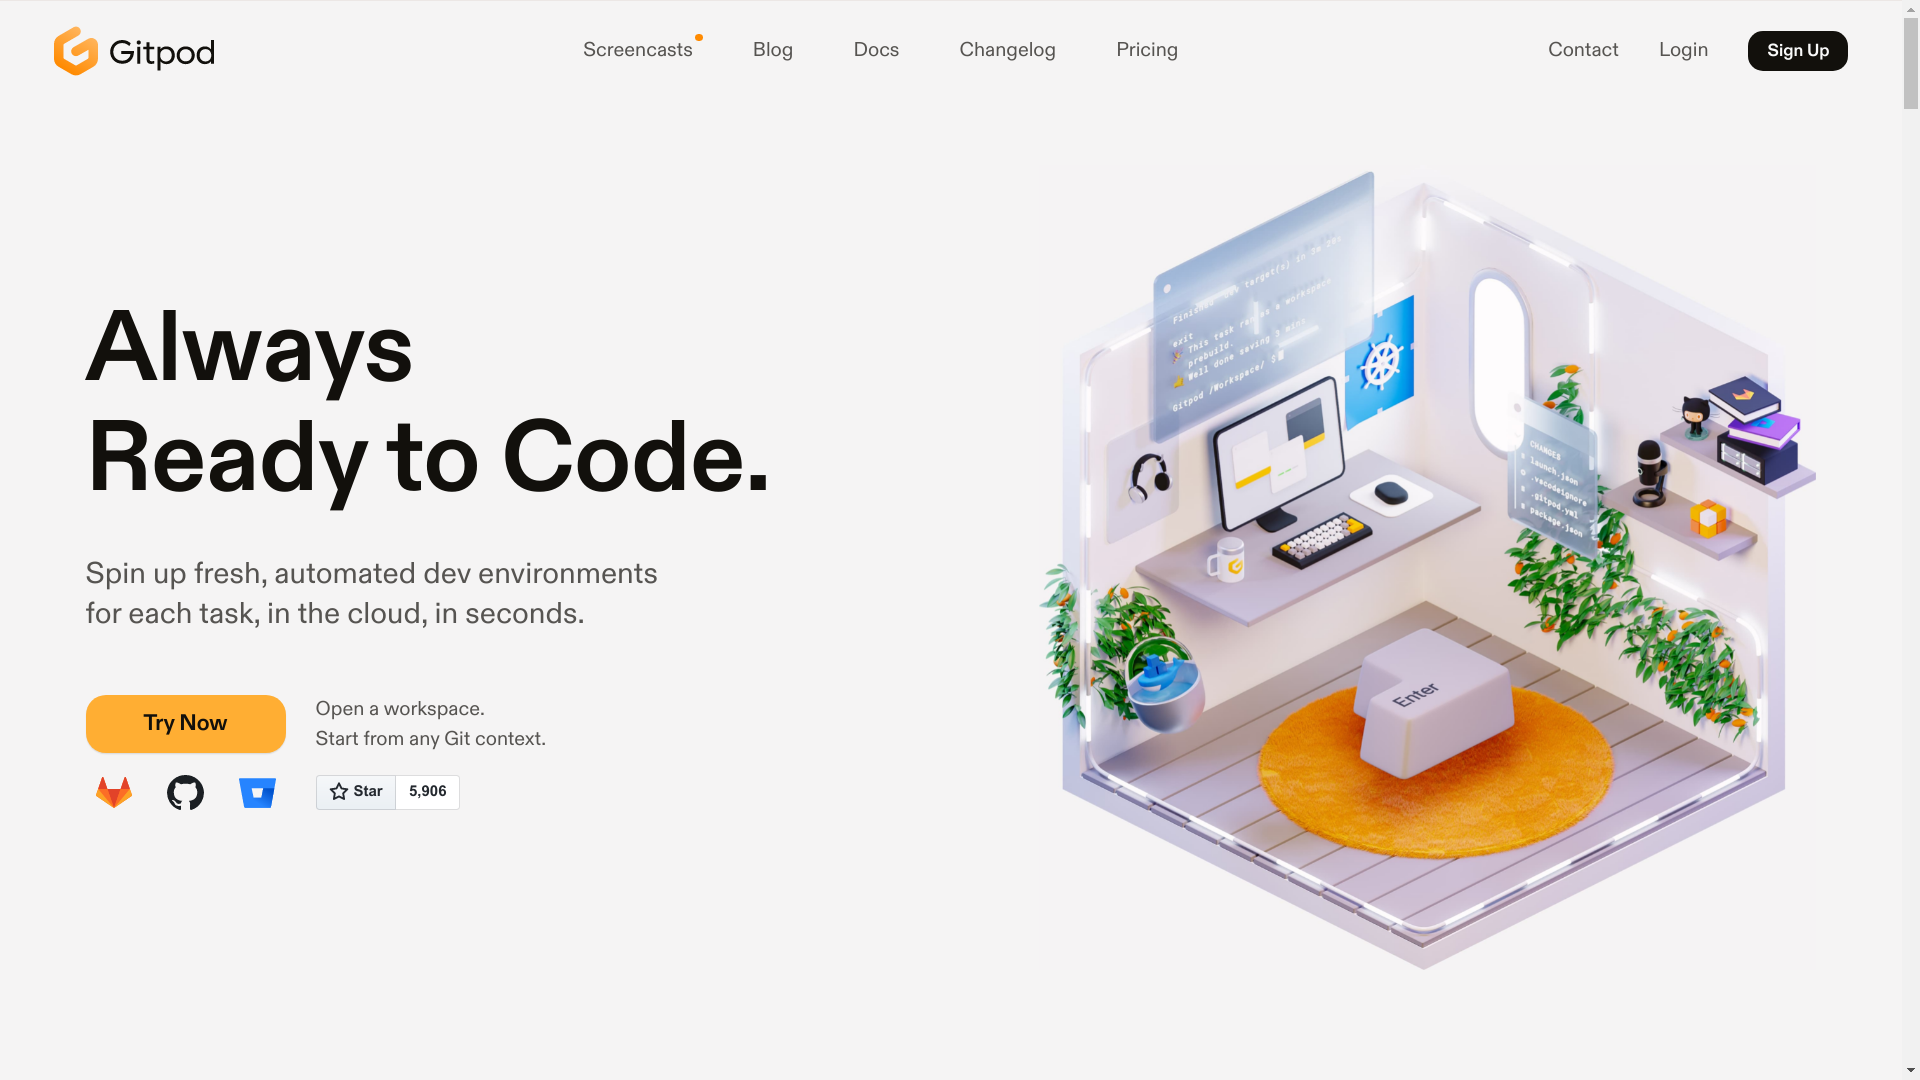
\includegraphics[width=.6\paperwidth]{images/homepage}
	      \end{figure}

	\item \url{https://gitpod.io/#https://github.com/cpp-review-dune/dune-book}
	      \begin{figure}[ht!]
		      \centering
		      
\includegraphics[width=.6\paperwidth]{images/opening}
	      \end{figure}
	      \begin{figure}[ht!]
		      \centering
		      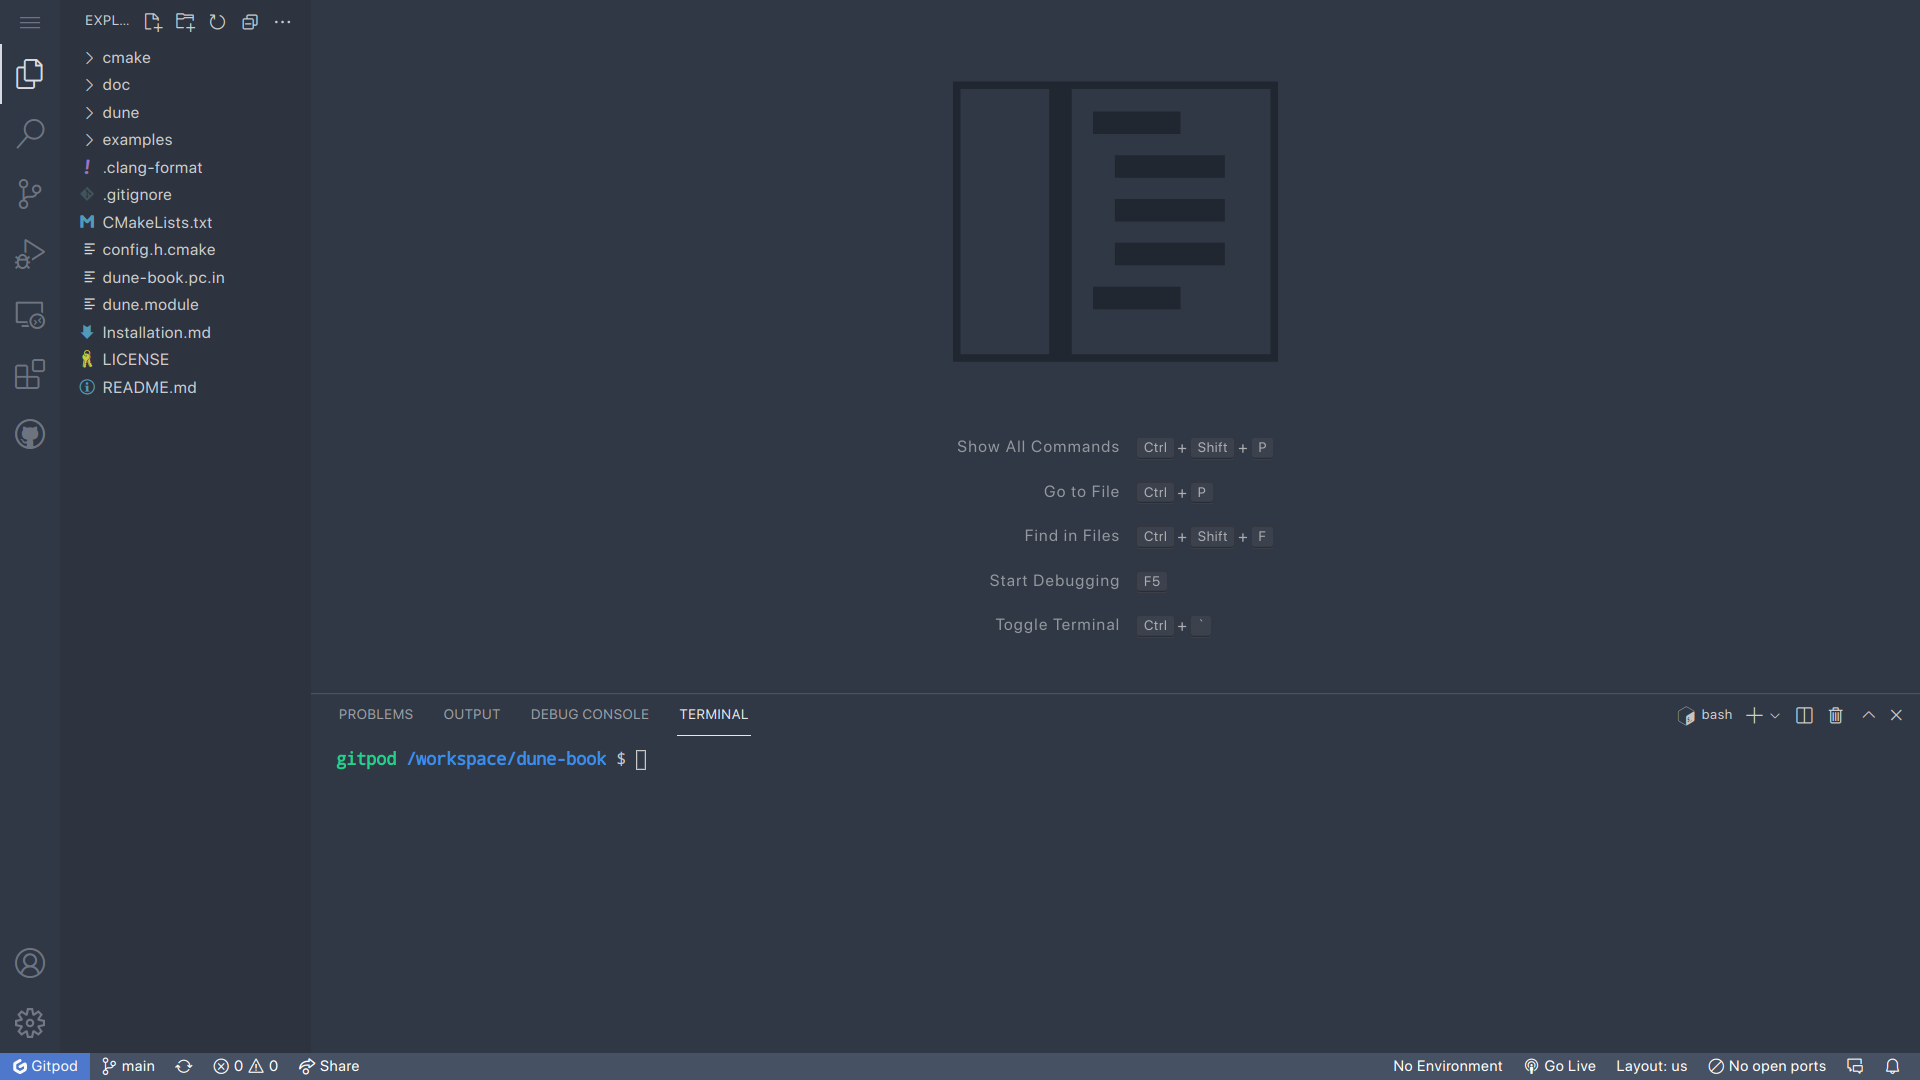
\includegraphics[width=.6\paperwidth]{images/editor}
	      \end{figure}
	      \begin{figure}[ht!]
		      \centering
		      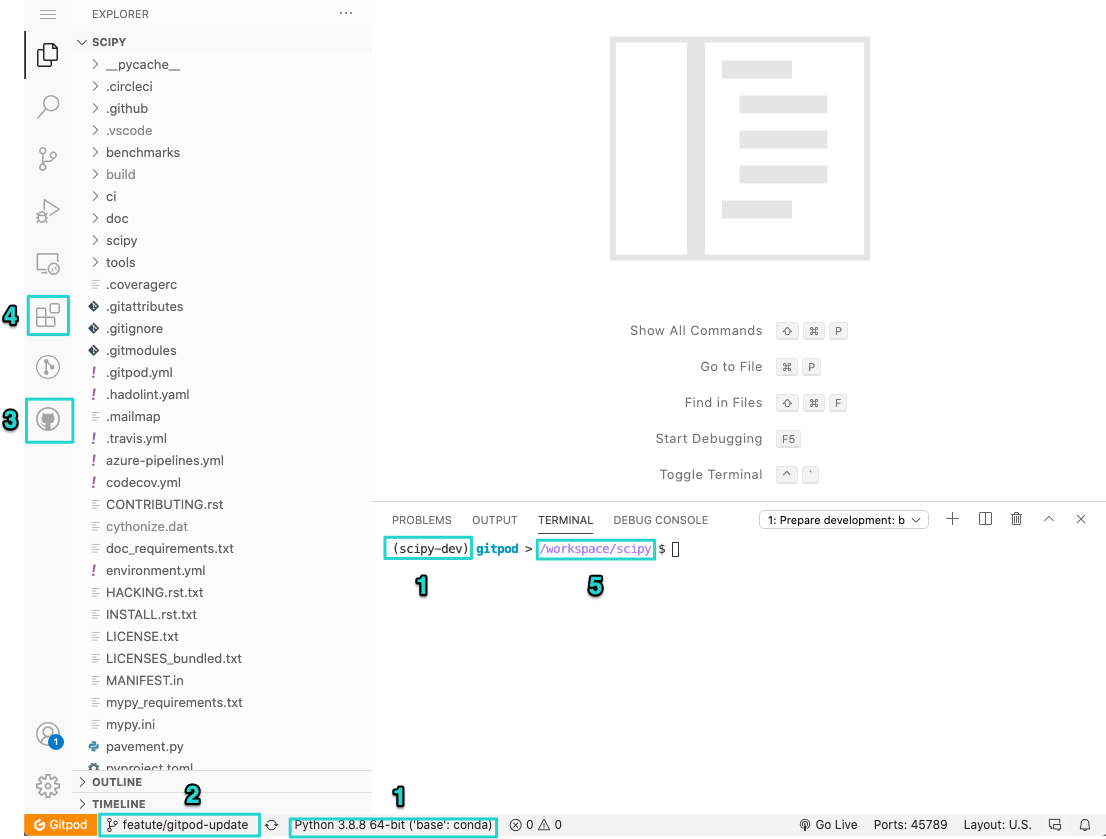
\includegraphics[width=.6\paperwidth]{images/gitpod-workspace}
		      \caption{Imagen de referencia.}
	      \end{figure}
	\item Crear un archivo, usar la terminal, crear carpetas, cambiar el tamaño de la letra (archivos/preferencias/configuración).
	\item Ejecute un programa en python, construya un proyecto en cmake.
	\item Cerrar el espacio de trabajo
	      % https://scipy.github.io/devdocs/dev/contributor/quickstart_gitpod.html
\end{enumerate}

% \section{Sistema de control de versiones}

\section{GitHub}

Para darse de alta en GitHub, necesitará completar el formulario \url{https://github.com/signup} y seguir la ayuda en línea \url{https://docs.github.com/es/get-started/quickstart} para configurar la herramienta git, crear repositorios, flujos de trabajo cooperativos.

\begin{figure}[ht!]
	\centering
	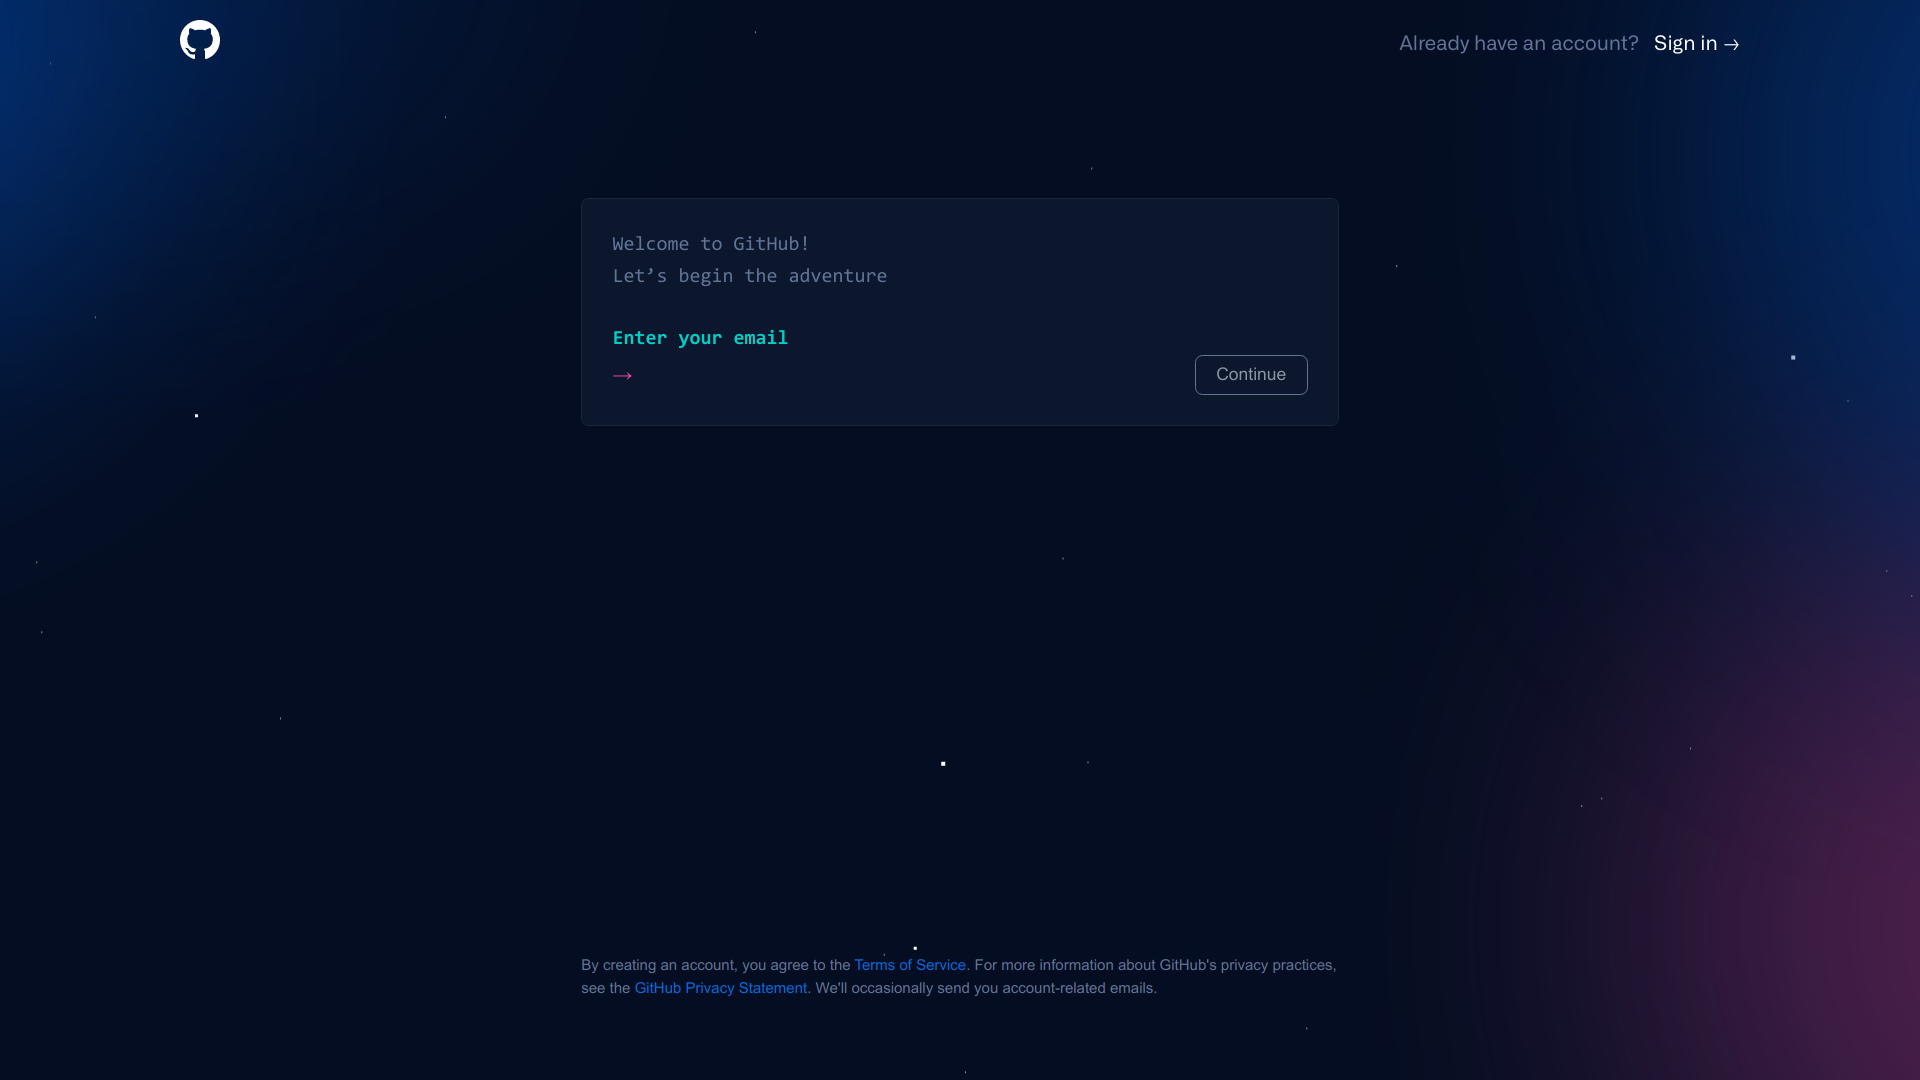
\includegraphics[width=.6\paperwidth]{images/signup}
\end{figure}

% Mostrar ejemplo con sparse-checkout, clonar repositorios, sincronizar un proyecto fork.

\section{GNU/Linux}

\section{Docker}

\url{https://docs.microsoft.com/es-es/dotnet/architecture/containerized-lifecycle/docker-terminology}

\begin{quote}
	Docker es un proyecto de código abierto para automatizar la implementación de aplicaciones como contenedores portátiles y autosuficientes que se pueden ejecutar en la nube o localmente.
	% \ref{msdocker}
	% TODO: Citar https://docs.microsoft.com/es-es/dotnet/architecture/containerized-lifecycle/what-is-docker
\end{quote}

\subsubsection{\texttt{docker run}}

\url{https://docs.docker.com/engine/reference/commandline/run}
\url{https://docs.docker.com/engine/reference/commandline/images}
\url{https://docs.docker.com/engine/reference/commandline/exec}

% Ejemplos

\begin{enumerate}
	\item Nos dirigiremos a \url{https://github.com/orgs/cpp-review-dune/packages} y seleccionaremos la imagen docker \texttt{dunepdelab}.
	      \begin{figure}[ht!]
		      \centering
		      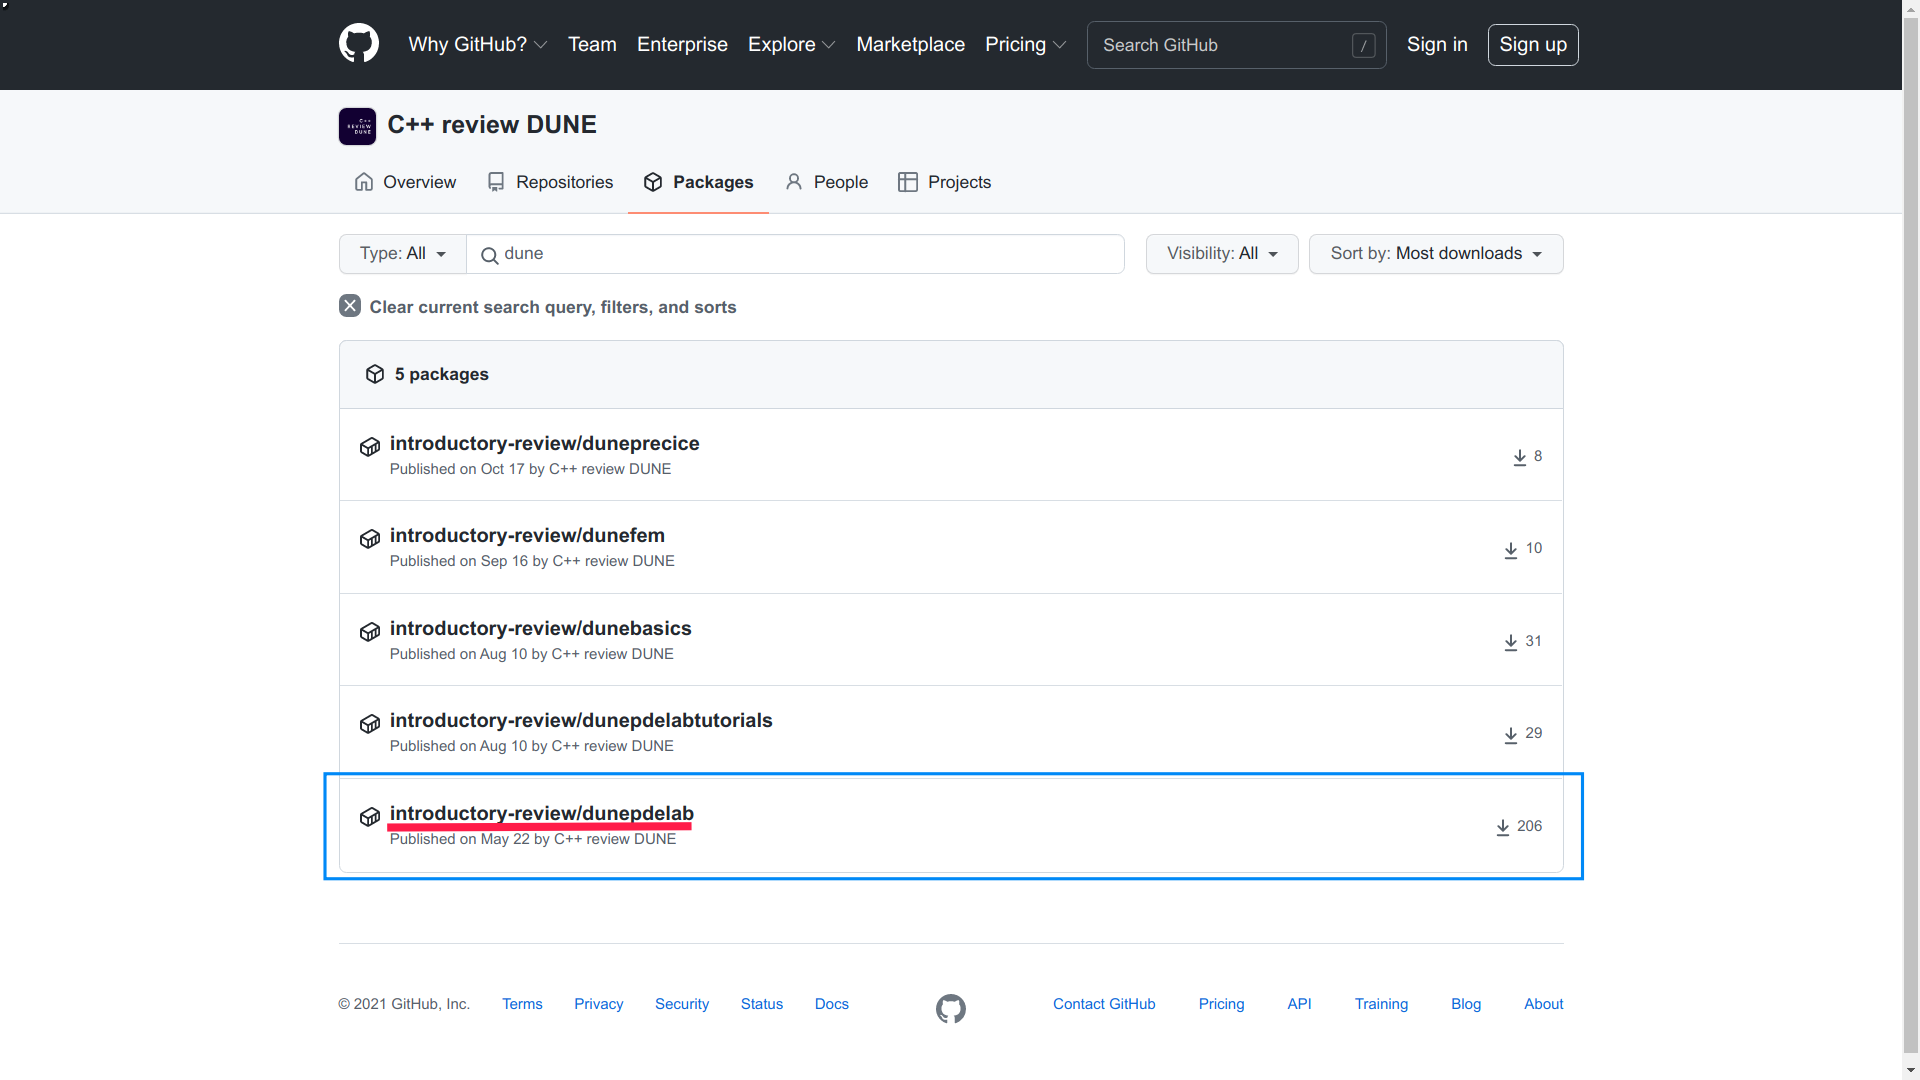
\includegraphics[width=.6\paperwidth]{images/imagedunepdelab}
	      \end{figure}
\end{enumerate}

\section{Testing e integración continua} % Yaml

\subsection{Debian based, Arch based}

% En caso que Gitpod soporte Arch, no mencionaré Ubuntu.

\section{Arch Linux}

% TODO: Errores frecuentes

Los principios de Arch Linux
% https://wiki.archlinux.org/title/Arch_Linux_(Espa%C3%B1ol)#Principios

Las diferencias entre Arch Linux y las demás.
% 1 párrafo
para los usuarios que ya han usado Linux pueden ver \url{https://wiki.archlinux.org/title/Pacman_(Espa%C3%B1ol)/Rosetta_(Espa%C3%B1ol)}
% https://wiki.archlinux.org/title/Arch_compared_to_other_distributions_(Espa%C3%B1ol)

Mostrar ejemplos, cómo se actualiza, cómo se instala, cómo se busca.

% Clonar, cambiar las ramas, subir y bajar los cambios.

\section{Introducción al empaquetamiento de software en Arch Linux}

